\section{本章小结}

本章介绍了导数。导数的基础是极限与连续,高中阶段不详细介绍极限与连续,所以对导数的推导和应用都比较简单,我只需要掌握求导公式和了解导数能用于求解极值即可。

%============================================================
\subsection{习题}

\begin{example}[拓广探索19,难度:$\star \star $]
已知函数$f\left( x \right) =ae^{2x}+\left( a-2 \right) e^x-x$。
\begin{enumerate}
    \item 讨论$f\left( x \right) $的单调性;
    \item 若$f\left( x \right) $有两个零点,求$a$的取值范围。
\end{enumerate}
\end{example}

解:

(1)对函数求导:
\begin{align*}
&f'\left( x \right) =2ae^{2x}+\left( a-2 \right) e^x-1 \\
&f''\left( x \right) =4ae^{2x}+\left( a-2 \right) e^x
\end{align*}
令$f'\left( x \right) =0$求得$e^x=1/a$,讨论:
\begin{itemize}
    \item 当$a=0$时,$f\left( x \right) =-2e^x-x$,显然单调递减;
    \item 当$a<0$时,$f'\left( x \right) <0$,显然单调递减;
    \item 当$a>0$时,求得极值点$x=\ln \frac{1}{a}$,$f''\left( \ln \frac{1}{a} \right) =\frac{2}{a}+1>0$,显然为极小值,函数先减后增。
\end{itemize}

(2)显然至少需要$a>0$,而且最小值必须小于0:
\begin{align*}
&\because f\left( \ln \frac{1}{a} \right) =a\frac{1}{a^2}+\left( a-2 \right) \frac{1}{a}-\ln \frac{1}{a}=1-\frac{1}{a}-\ln \frac{1}{a}<0 \\
&\therefore 1-\frac{1}{a}<\ln \frac{1}{a} \\
&\therefore \frac{1}{a}>1
\end{align*}
得到取值范围$0<a<1$,$a$分别取0.5、0.8、1时$f\left( x \right) $的图形如下:

\begin{figure}[h]
\centering
\begin{minipage}{.32\textwidth}
\centering
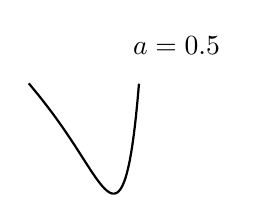
\begin{tikzpicture}[line join=round, scale=0.4]
\mydrawxy{-3}{3}{-2}{3}
\draw[thick,domain=-2:1.5,samples=200] plot (\x,{(0.5)*exp(2*\x)+(0.5-2)*exp(\x)-\x});
\coordinate[label=right:{$a=0.5$}] (t) at (1,3);
\end{tikzpicture}
\end{minipage}
\begin{minipage}{.32\textwidth}
\centering
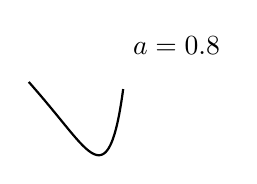
\begin{tikzpicture}[line join=round, scale=0.4]
\mydrawxy{-3}{3}{-2}{3}
\draw[thick,domain=-2:1,samples=200] plot (\x,{(0.8)*exp(2*\x)+(0.8-2)*exp(\x)-\x});
\coordinate[label=right:{$a=0.8$}] (t) at (1,3);
\end{tikzpicture}
\end{minipage}
\begin{minipage}{.32\textwidth}
\centering
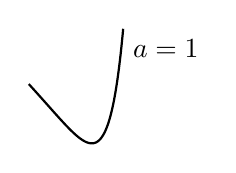
\begin{tikzpicture}[line join=round, scale=0.4]
\mydrawxy{-3}{3}{-2}{3}
\draw[thick,domain=-2:1,samples=200] plot (\x,{(1)*exp(2*\x)+(1-2)*exp(\x)-\x});
\coordinate[label=right:{$a=1$}] (t) at (1,3);
\end{tikzpicture}
\end{minipage}
\end{figure}

\begin{tcolorbox}
本题没有难度。函数形状的讨论都是针对其一阶和二阶导数的分段讨论,讨论的是另两个函数。
\end{tcolorbox}




